Resumen de las principales estadísticas descriptivas de las variables relevantes en los logs de navegación.
Análisis de la distribución de los datos, incluyendo medidas de centralidad y dispersión.
Haciendo uso de la librería pandas podemos obtener informacion respecto al dataframe, cantidad de valores únicos y calcular estadísticas descriptivas:

Podemos obtener informacion respecto a la cantidad de valores faltantes de cada dataframe que se está utilizando, los cuales son \textbf{36853}:

\begin{figure}[H]
    \begin{minipage}[t]{0.9\textwidth}
        \caption{Datos faltantes dataframes.}
        \label{descripcion_dataframe}        
    \end{minipage}

    \vspace{10pt}

    \begin{minipage}[b]{0.85\textwidth}
        \centering
        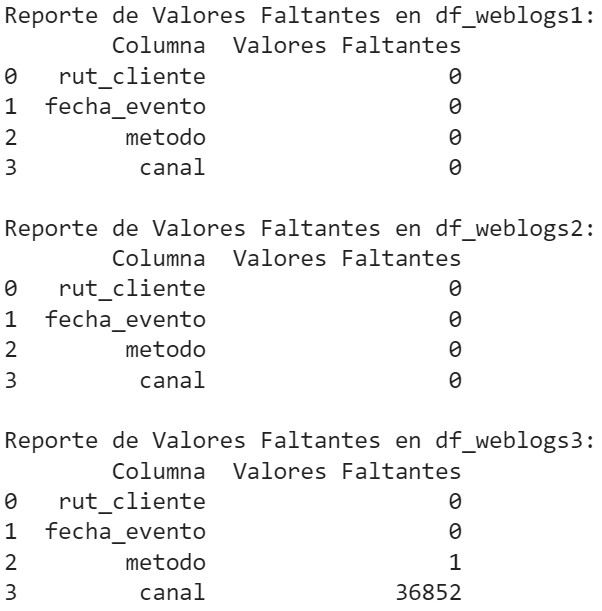
\includegraphics[width=\textwidth]{img/valores faltantes datasets.jpg}        
    \end{minipage}

    \begin{minipage}[t]{0.9\textwidth}
        Fuente: Elaboración propia.
    \end{minipage}
\end{figure}

\begin{itemize}
    \item \textbf{rut cliente:} Contiene datos de tipo int64.
    \item \textbf{fecha evento:} Contiene datos de tipo object.
    \item \textbf{metodo:} Contiene datos de tipo object.
    \item \textbf{canal:} Contiene datos de tipo object.
\end{itemize}

Además se puede conocer la cantidad de valores únicos que posee cada una de las columnas de los 2 datasets:

Dataset 1:

\begin{itemize}
    \item \textbf{rut cliente:} Contiene 40125 valores únicos.
    \item \textbf{fecha evento:} Contiene 80181 valores únicos.
    \item \textbf{metodo:} Contiene 81254 valores únicos.
    \item \textbf{canal:} Contiene 81254 valores únicos.
\end{itemize}

Dataset 2:

\begin{itemize}
    \item \textbf{rut cliente:} Contiene 40224 valores únicos.
    \item \textbf{fecha evento:} Contiene 80470 valores únicos.
    \item \textbf{metodo:} Contiene 81546 valores únicos.
    \item \textbf{canal:} Contiene 81546 valores únicos.
\end{itemize}

La librería pandas ofrece una buena cantidad de estadísticas descriptivas gracias a su función .describe, las cuales se muestran a continuación:
\begin{itemize}
    \item \textbf{Recuento (count):} Calcula el número de valores no nulos en cada columna. \textbf{count: 58009.000000} valores no nulos.
    \item \textbf{Media (mean):} Calcula la media de las columnas numéricas. \textbf{mean: 504.854902} 
    \item \textbf{Desviación estándar (std):} Calcula la desviación estándar de las columnas numéricas. \textbf{std: 553.964179}
    \item \textbf{Mínimo (min):} Calcula el valor mínimo de las columnas numéricas. \textbf{min: 1.000000}
    \item \textbf{Cuartiles:} Calcula los cuartiles de las columnas numéricas 
    \begin{itemize}
        \item \textbf{25\%: 8.000000}
        \item \textbf{50\%: 303.000000}
        \item \textbf{75\%: 884.000000}
    \end{itemize}
    \item \textbf{Máximo (max):} Calcula el valor máximo de las columnas numéricas. \textbf{max: 1815.000000}
\end{itemize}
%Identificación de cualquier valor atípico o dato faltante en los registros y discusión sobre cómo se manejarán estos casos.